\documentclass[11pt,letter]{article}

\setlength{\topmargin}{0in}
\setlength{\headheight}{0in}
\setlength{\headsep}{0in}
\setlength{\textheight}{9in}
\setlength{\oddsidemargin}{0in}
\setlength{\textwidth}{6.5in}

\usepackage{amsmath}
\usepackage{amsfonts}
\usepackage{amssymb}
\usepackage{appendix}

\usepackage{epsfig}
\title{A Framework for Personalized Photograph Quality Assessment}
\author{
K. Armin Samii \\
ksamii@ucsc.edu
\and
Uliana Popov \\
uliana@soe.ucsc.edu}
\date{May 13, 2011}

\begin{document}
\maketitle
\begin{abstract}
Photograph quality assessment can help aid home users in managing their personal collections in several ways, including deleting low-quality images and browsing for high quality images. Recent research has aimed to automatically rate image quality, but such methods are not yet perfected. In this paper, we propose a framework for quickly developing and testing new features to accelerate the progress of this research. We have two types of features: \textit{high-level features} that are subjective qualities which humans can easily understand, such as exposure quality or sharpness; \textit{low-level features} that are objective calculations which are produced algorithmically, like edge width or number of dark pixels. We use machine learning techniques to learn how each of these relate to image quality. 
Our framework is intended to be used by both developers and end-users (photographers). 
The model allows for an application developer to easily add new features, both low-level and high-level. Additionally, we allow the photographer using the application to modify the importance of each high-level features based on personal preferences.
We implement our framework in a real image quality assessment application and show improvement over the untrained application.

\end{abstract}

\section{Problem Statement}
A photographer wishes to automatically rate his photograph collection based on his personal preferences. There are several papers dedicated to solving this problem using machine learning\cite{springerlink:10.1007/11744078_23}\cite{springerlink:10.1007/978-3-642-10543-2_23}\cite{Yeh:2010:PPR:1873951.1873963}. To accelerate research in the area, we need to develop a framework for developers (researchers) to quickly train new features extracted from photographs.

There are two audiences we are trying to serve in this work: (1) the photographer using the application, and (2) the developer producing the application. In other words, we want to make it as easy as possible for the developer to serve the photographer.

To serve (1) the photographer, we want to allow him to choose which features he personally finds important (see Section \ref{abstraction}). To serve (2) the developer, we want to allow her to be able to add new features with ease (see Section \ref{easeofprogramming}). Figure \ref{fig:flowchart} visualizes these ideas.

\begin{figure*}[b!]
  \centering
    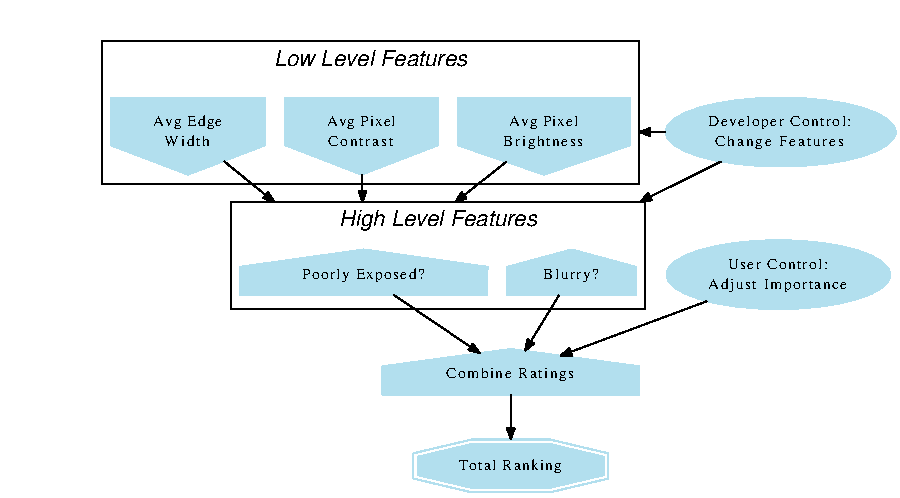
\epsfig{file=mlflowchart.pdf,width=14cm}
  \caption{An example flowchart. Here, the application computes three low-level features. All three combine to rate the two high-level features: blurriness and exposure. The developer controls which features are present. The photographer's personal preferences can change the default weights on high-level features.}
  \label{fig:flowchart}
\end{figure*}

\subsection{Helping the Photographer Personalize Ratings}
\label{abstraction}
While it is difficult for a human to interpret the meaning of low-level features, high level features are intended for human understanding. Thus, we use high-level features as a layer of abstraction: Instead of asking the photographer to change the default weights on low-level features, we present them with high-level features. But, this presents the following two questions:


\begin{figure}
\centering
\resizebox{12cm}{!}{
\begin{tabular}[t]{| l || c | c |}
 \hline
 Low Level Feature & Default Learned Weights & Penny's Weights \\ 
 \hline
Exposure & .4 & .2 \\ 
 \hline
In-focus & .6 & .8 \\ 
 \hline
\end{tabular}
}
\caption{Example of a photographer changing the default weights. The weights correspond to how much each high-level feature contributes to the overall rating. Photographer Penny does not mind underexposed images, so she lowers the weight of the "Exposure" high-level feature. "Blur" is updated accordingly.}
\label{fig:weighttable}
\end{figure}

\begin{enumerate}
\item \textbf{How important is each high-level feature to the overall rating of a photograph?}

%This question is relevant to the photographer. As an example:

%Photographers Penny and Quinn want to automatically rate their photographs so they can ignore those with low ratings and save some time when browsing their collections.
For example: Photographer Penny takes pictures at concerts so she doesn't mind slightly underexposed images. Penny will decrease the default weight on the high-level "exposure" feature. The weights on the other high level features will be updated accordingly. Figure \ref{fig:weighttable} demonstrates this.

\item \textbf{How does each low-level feature affect the ranking of a high-level feature?}

%This  question is relevant to the developer. As an example:

For example: Programmer Pete calculates three low-level features per image: average width of edges, average pixel contrast, and average pixel brightness. He wants to use these low-level features to see if an image is blurry or poorly exposed. Our framework will train multiple SVRs using the three low-level features. Each SVR will determine the relationship between low-level and high-level features.

\end{enumerate}

\subsection{Helping the Developer Make Progress}
\label{easeofprogramming}
%The Developer will want 
When a developer needs to add more features as research progresses. There are two types of features which can be added:
\begin{enumerate}
\item \textbf{Adding low-level features}

Say Programmer Pete calculates the number of vibrant pixels in an image. He should be able to insert this feature into the program with ease. The photographer would be unaware of any changes other than an improvement in accuracy.

\item \textbf{Adding high-level features}

Say Programmer Pete decides that Saturation is important. Then he will want to see just how much saturation is relevant to image quality. The end-user photographers will be aware of this new change, and can adjust the high-level weights accordingly.
\end{enumerate}

\section{Introduction}
To solve the problem presented, one might try to directly train low-level features to rate image quality. However, photograph quality is highly subjective and this approach does not allow a photographer to personalize the importance of each feature.

So instead, one might try to directly compute high-level features. However, this method risks using a poor algorithm to calculate a high-level feature, and thus sacrifices accuracy. (It is hard to calculate "color quality;" it is easy to calculate the number of saturated pixels.)

We thus propose a hybrid method which separately trains low-level and high-level features. This method allows (1) the photographer to personalize each high-level feature's importance, and (2) the developer to have multiple low-level calculations to rate each high-level feature. Further, the developer can (3) dynamically change which features are used (both low-level and high-level).

To answer the first question presented in Section \ref{abstraction}, we use a Linear Regression learning model. We chose a Linear Regression because it allows for the photographer to adjust the importance of each feature without retraining the model.

For the second question, the user does not have control over the default weights, so we use the more accurate model of Support Vector Regression Machines (SVRs)\cite{springerlink:10.1023/B:STCO.0000035301.49549.88}. We train one SVR per high-level feature, resulting in an ensemble of SVRs, each trained to a different high-level feature. We chose this model because SVRs, in general, have higher accuracy than a Linear Regression. We use an ensemble because each one can specialize to a certain feature, allowing for our Linear Regression to exist. %ZZZ: I added explanation about why we chose- is it too wordy now? 
%UUU. No. it is good now

When the developer adds a new low-level feature, every SVR in the ensemble is updated. When the developer adds a high-level feature, another SVR is added to the ensemble. These methods are described in detail in Section \ref{methods}. The high-level features for the images in the training set are labeled by surveying Amazon Mechanical Turk\footnote{MTurk: http://www.mturk.com} users (Turkers). Figure \ref{fig:turkexample} shows an example of what Turkers are asked.

\begin{figure*}[h!]
  \centering
    \fbox{
      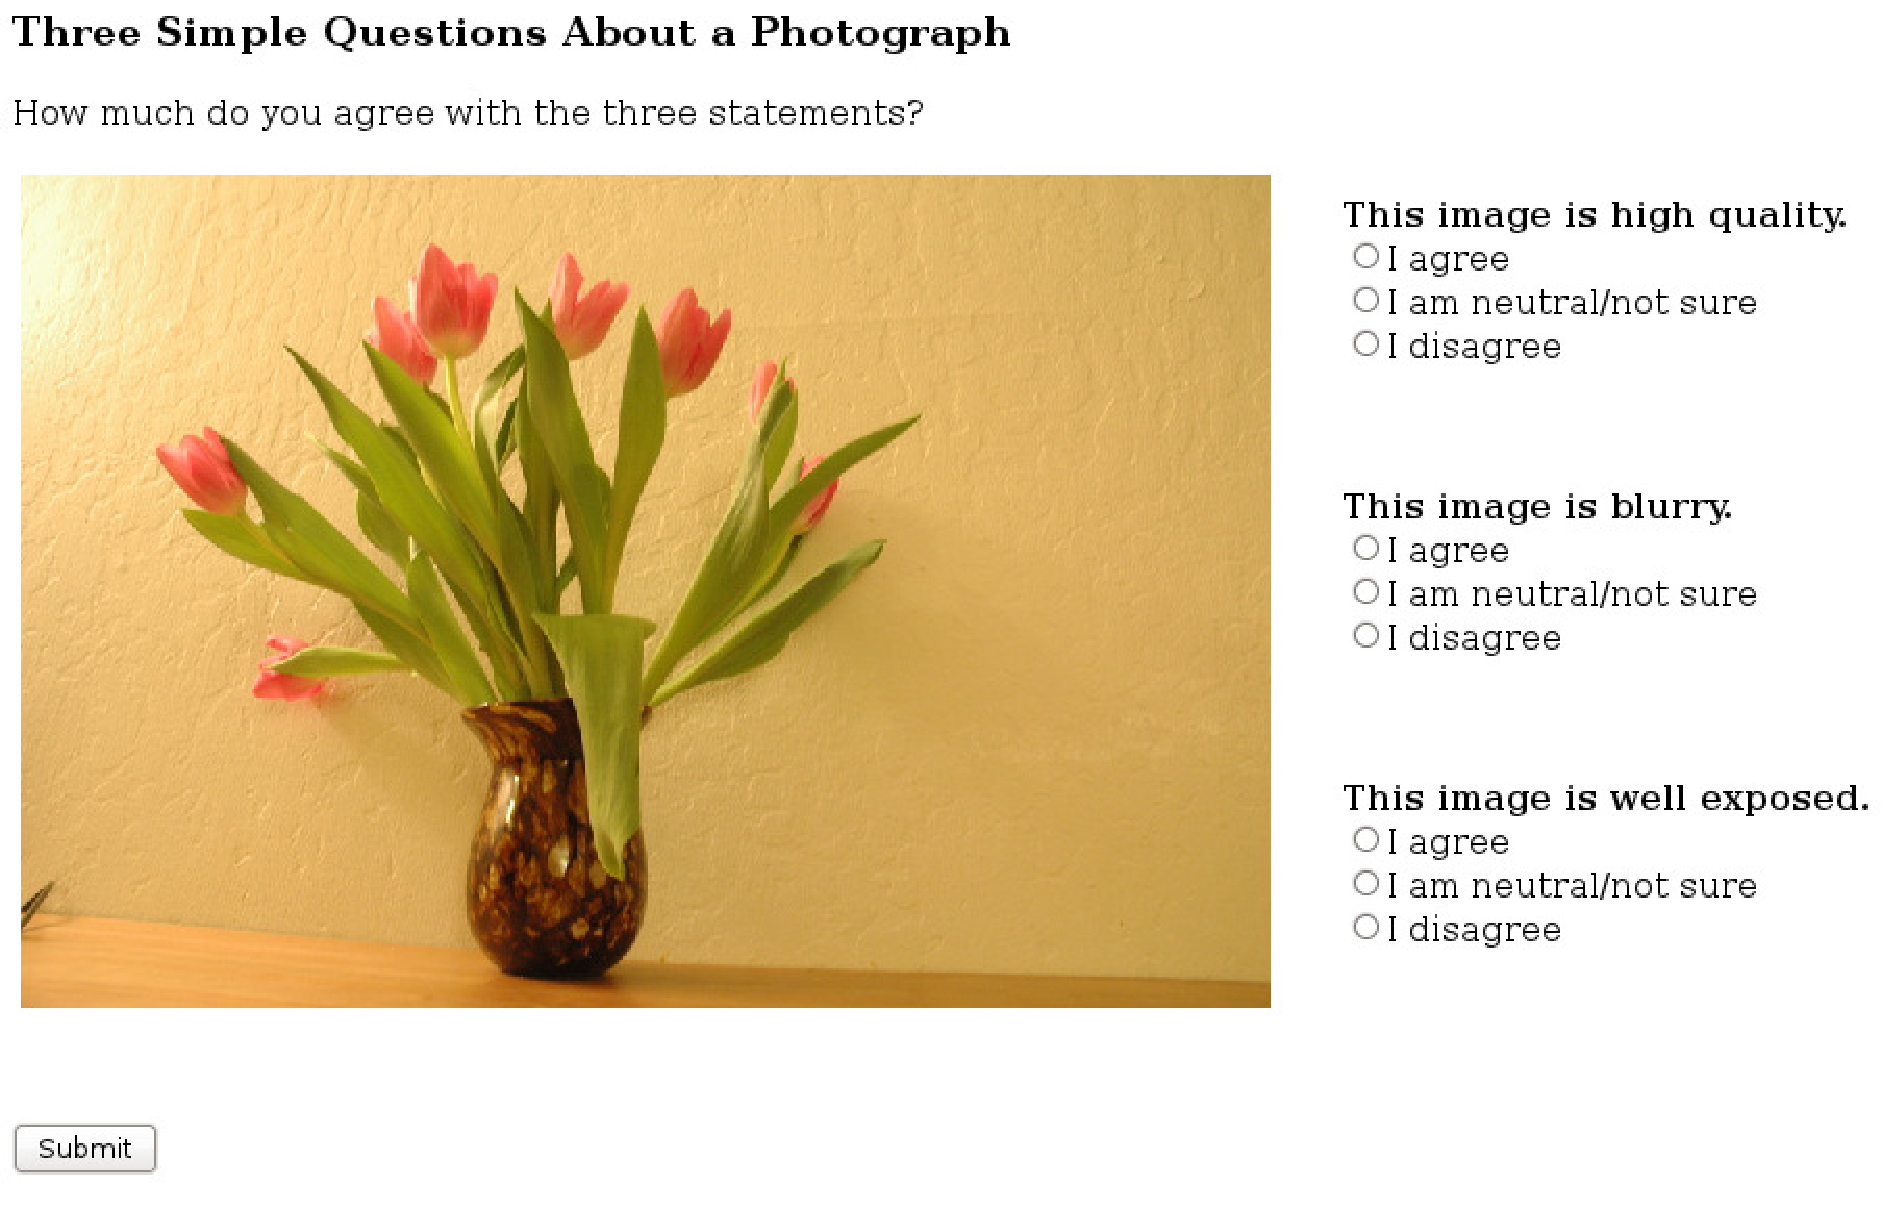
\epsfig{file=turkexample.pdf,width=17cm}
    }
  \caption{This is what Turkers see when rating the image. Here, there are two high level features: blur quality and exposure quality. 
That are determined by two last statements on the right.
The first statement (``This image is high quality'') is the ground truth. See Section \ref{turkdata} for details.}
  \label{fig:turkexample}
\end{figure*}

\section{Related Work}
Tong and Chang\cite{Tong:2001:SVM:500141.500159} use Support Vector Machines to search a database of images quickly by choosing images that are visually similar, which abstracts the features from the user completely.

The Personalized Photograph Ranking and Selection System\cite{Yeh:2010:PPR:1873951.1873963} computes high-level features directly and uses ListNet\cite{Cao:2007:LRP:1273496.1273513} to find a ranking. However, this does not allow for the training of several low-level features to produce a single high-level feature, which can increase the overall accuracy.

\section{Data}

There are two sets of data used, both of which are learned independently.

\subsection{User-Produced Data}
\label{turkdata}
The initial set of data was produced by giving Turkers a simple statement for each high level feature, and asking if they agreed. Our primary ground-truth statement for each image is:

``This image is high quality.''

We present this to five Turkers and ask them to choose one of three options:

\begin{itemize}
\item ``Agree'' (+1 point)
\item ``Neutral'' (+.5 points)
\item ``Disagree'' (+0 points)
\end{itemize}
The points are then averaged across the five Turkers' responses to obtain a final score.

We repeat this process for each high level feature, with statements such as ``This image is in focus'' and ``This image is well-exposed.'' The data then looks as shown in Figure \ref{fig:turktable}.

\begin{figure}
\centering
\resizebox{12cm}{!}{
\begin{tabular}[t]{| c || c || c | c | c | l | }
 \hline
 & High Quality & In focus & Well exposed & Good saturation & \ldots \\ 
 \hline
Image 1 & .5 & .3 & 1 & .8 & \ldots \\ 
 \hline
Image 2 & .1 & ? & .4 & .4 & \ldots \\ 
 \hline
Image 3 & .9 & .8 & .6 & ? & \ldots \\ 
 \hline
\vdots & \vdots & \vdots & \vdots & \vdots & $\ddots$ \\
 \hline
\end{tabular}
}
\caption{The information collected from Amazon Mechanical Turk, showing example values for high-level questions. There are some values missing, indicated by a question mark (?), in case we do not have information from Turkers about that high-level feature. We discuss how to handle this in Section \ref{llfeat}.}
\label{fig:turktable}
\end{figure}

\\
\\

During training, the overall rating for an image is learned indirectly, through a linear regression of the high-level features' SVRs.

\subsection{Application-produced data}
The developer chooses which low-level features to calculate. Each of these calculations is used in all the SVRs to obtain ratings of the high-level features. Recall that each SVR is trained to produce a numerical prediction for a single high-level feature.


\section{Implementation of Training Methods}
\label{methods}

There are two steps to the learning process. First, we learn the importance of each high-level feature on the overall image rating. These are the default weights which can be modified by the photographer. Then, we learn how each low-level feature affects each high-level feature.

\subsection{Learning High-Level Features}
We use a linear regression to train each high level feature. For this, we do not take into account any low-level features. The error function is defined as:
\[
E=\displaystyle\sum\limits_{i=0}^N R_i-Z_i
\]
Where $E$ is the error, $N$ is the number of images in the training set, $R_i$ is the overall rating obtained from Turkers for image $i$, and $Z_i$ is as follows:
\[
Z_i=\displaystyle\sum\limits_{f=0}^M w_f \cdot r_{i,f}
\]
Where $M$ is the number of high-level features, $w_f$ is the weight of feature $f$, and $r_{i,f}$ is the Turkers rating of feature $f$ on image $i$.

We minimize this error function over all $w_i$, ensuring
\[
\displaystyle\sum\limits_{f=0}^M w_f = 1
\]


\subsection{Learning Low-Level Features}
\label{llfeat}
We use an ensemble of Support Vector Regression Machines (SVRs) to learn low-level features. Each SVR is trained to learn a single high-level feature (e.g. the last three columns of Figure \ref{fig:turktable}). The number of SVRs is equal to the number of high-level feature ratings provided by Turkers, as shown in Section \ref{turkdata}.

We want to be able to ask Turkers new questions to use as high-level features, and add an SVR to the ensemble. If we do not retrain on every image used as training data, we need to handle missing data.

The solution is straightforward: If we do not have Turk data for a certain high-level feature, we do not train on that image for the SVR. Note that to learn high-level features, we can only use complete rows (images with no missing values).

We use an SVR with soft margins to allow for some noise in our data. We also normalize the low level feature values and the high level feature labels. Support Vector Regression machines work as follows: We want to find a function $S$ such that

\[
S(x)=\langle w, x\rangle + b, x\in \mathbb{R}^d, w\in \mathbb{R}^d, b\in \mathbb{R}
\]

We find $w$ by minimizing the function:

\[
\frac{1}{2}||w^2||+C\displaystyle\sum\limits_{i=0}^l(\xi_i+\xi_i*)
\]

Where $C$ is a parameter which determines the trade-off between good generalization and high accuracy on the training set (we set $C=5$); $l$ is the number of training examples; and $\xi_i$ and $\xi_i*$ are the ``slack variables'' which allow for noise in the data, and are defined in the following two constraints to the above formula:

\[
y_i-\langle w,x_i\rangle-b\leq \epsilon + \xi_i
\]
and
\[
-y_i+\langle w,x_i\rangle+b\leq \epsilon + \xi_i*
\]

Where each $(x_i, y_i)$ pair is a labeled training example, and $\epsilon$ is a parameter representing the acceptable deviation from the target $y_i$. We set $\epsilon=.1$, allowing a relatively large error margin of .1 (about 10\% on our normalized data) because of the noise in both the input $x_i$ (the low level features calculated) and the labels $y_i$ (the high level feature values obtained from Turk).

We use a radial-based kernel function in lieu of the dot product $\langle w,x_i\rangle$, so that:
\[
\langle w,x_i\rangle = exp(-\gamma |w-x|^2)
\]

Where we set $\gamma=1$.

A more detailed discussion on Support Vector Regression Machines is discussed in Smola and Scholkopf's overview paper\cite{springerlink:10.1023/B:STCO.0000035301.49549.88}.

\subsection{Output on new images}
After training, the rating $O_i$ of a new image $i$ is as follows:
\[
O_i=\frac{1}{M}\displaystyle\sum\limits_{f=0}^Ma_f \cdot w_f \cdot S_f(i)
\]
Where $M$ is the number of high-level features, $a_f$ is the personalized weight adjustment for feature $f$, $S_f$ is the output of the Support Vector Regression for high level feature $f$ on image $i$, and the other variables are as defined above. $a_f$ is subject to:
\[
\displaystyle\sum\limits_{f=0}^M a_f = 1
\]


\section{Adding Features}
Here, we show the ease of adding new features in our application. Training data is saved to a file and loaded when the application begins, so training only occurs when the user requests it using our GUI (Appendix \ref{gui}).

\subsection{New High Level Features}
To add a new high level feature, the developer must:

\begin{enumerate}
\item Obtain MTurk data, as shown in Section \ref{turkdata}.
\item Place the .CSV file (provided by MTurk) in the \texttt{trainingdata/} directory.
\end{enumerate}

Then, use the GUI to retrain; the SVR and Linear Regression function are automatically updated. The application automatically combines all .CSVs in the directory and extracts labels. It handles multiple files containing high-level feature labels for the same image. See Figure \ref{fig:turktable} for the data extracted.

\subsection{New Low Level Features}
If a new value is produced by the application, it can be added to the training set with the following line of code (C++):

\texttt{features.push\_back(value);}

Where \texttt{features} is the vector (array) of low-level features and \texttt{value} is the new value. Then, use the GUI to retrain; the SVR is automatically updated.

\section{Results}
We show our accuracy by predicting on two data sets. Both of these have ground truth ratings from Turk. Because we want to show how machine learning improved our original application\cite{imagesorter} which did not use Machine Learning, we focus on how much \textit{better} we do with machine learning than we did by guessing parameters.

By implementing machine learning, we had an added resource restriction: to train, we needed to calculate low-level features for several hundred images quickly. We had to thus remove a lot of complexity in the calculations of the low-level features, reducing the computation time from about two minutes per image to about ten seconds (on a single core Intel processor at 4.5Ghz). We show that we still improve over our untrained algorithm.

We ignore any Photographer Preferences in these results, and use the default weights learned by the Linear Regression.

\section{Conclusion and Future Work}
We have developed a framework for continuing research on rating image quality. First, a developer calculates \textit{low-level feature} values based on image data. Turk users provide answers to \textit{high-level features}, as well as an overall rating of the quality.

Using linear regression, we determine which high-level features are most correlated with the overall rating. Then, we use train one Support Vector Regression per high-level feature, and using the weights from the linear regression, obtain a final value for the image.

We implement the framework in our previous research which calculates low-level features. Our accuracy increases using the machine learning techniques (as compared to arbitrarily hypothesized weights for both steps of learning: low-level to high-level and high-level to overall quality).

Future work should implement a discriminant analysis to remove irrelevant low-level features from the SVRs of high-level features, because unrelated features lower the accuracy of an SVR. For example, vibrant pixels (low-level) would have no effect on blur amount (high-level), so the extra dimension is essentially random.

An online learning algorithm could also be implemented as follows: for every image that the algorithm predicts on, automatically query MTurk for labels, and retrain the SVRs accordingly.

\subsection{Low Quality Data Set}
Previously, out of 74 low-quality photographs, we gave 63 a low rating (less than .5). After training our algorithm, we gave 61 a low rating- about the same, but with a huge increase in processing time.

\subsection{Average Quality Data Set}
For completeness, we must also show that we do not rate high-quality and average-quality images poorly. We use INRIA's publicly-available "Original Image" dataset\cite{JDS08} for these images. Previously, we had correctly gave 135 out of 157 a high rating (greater than .5), 
which is almost 86\% accuracy. After training, we correctly gave 139 a high rating,
which is equal to a 88.5\%.
This is a slight improvement in accuracy, again with a significant improvement in processing time.

\appendix
\section{Graphical User Interface}
This section shows the GUI used for training and prediction.

\subsection{Training}
There are two ways to gather training data. By default, the last used SVR ensemble and Linear Regression function are loaded. The user can choose to train on new data by selecting a set of images (Figure \ref{fig:learnpage}). The application looks through all the MTurk data files for matching high-level labels and trains on these images. It ignores unlabeled images, and warns the user if none of the selected images have labels.

\begin{figure*}[h!]
  \centering
    \fbox{
      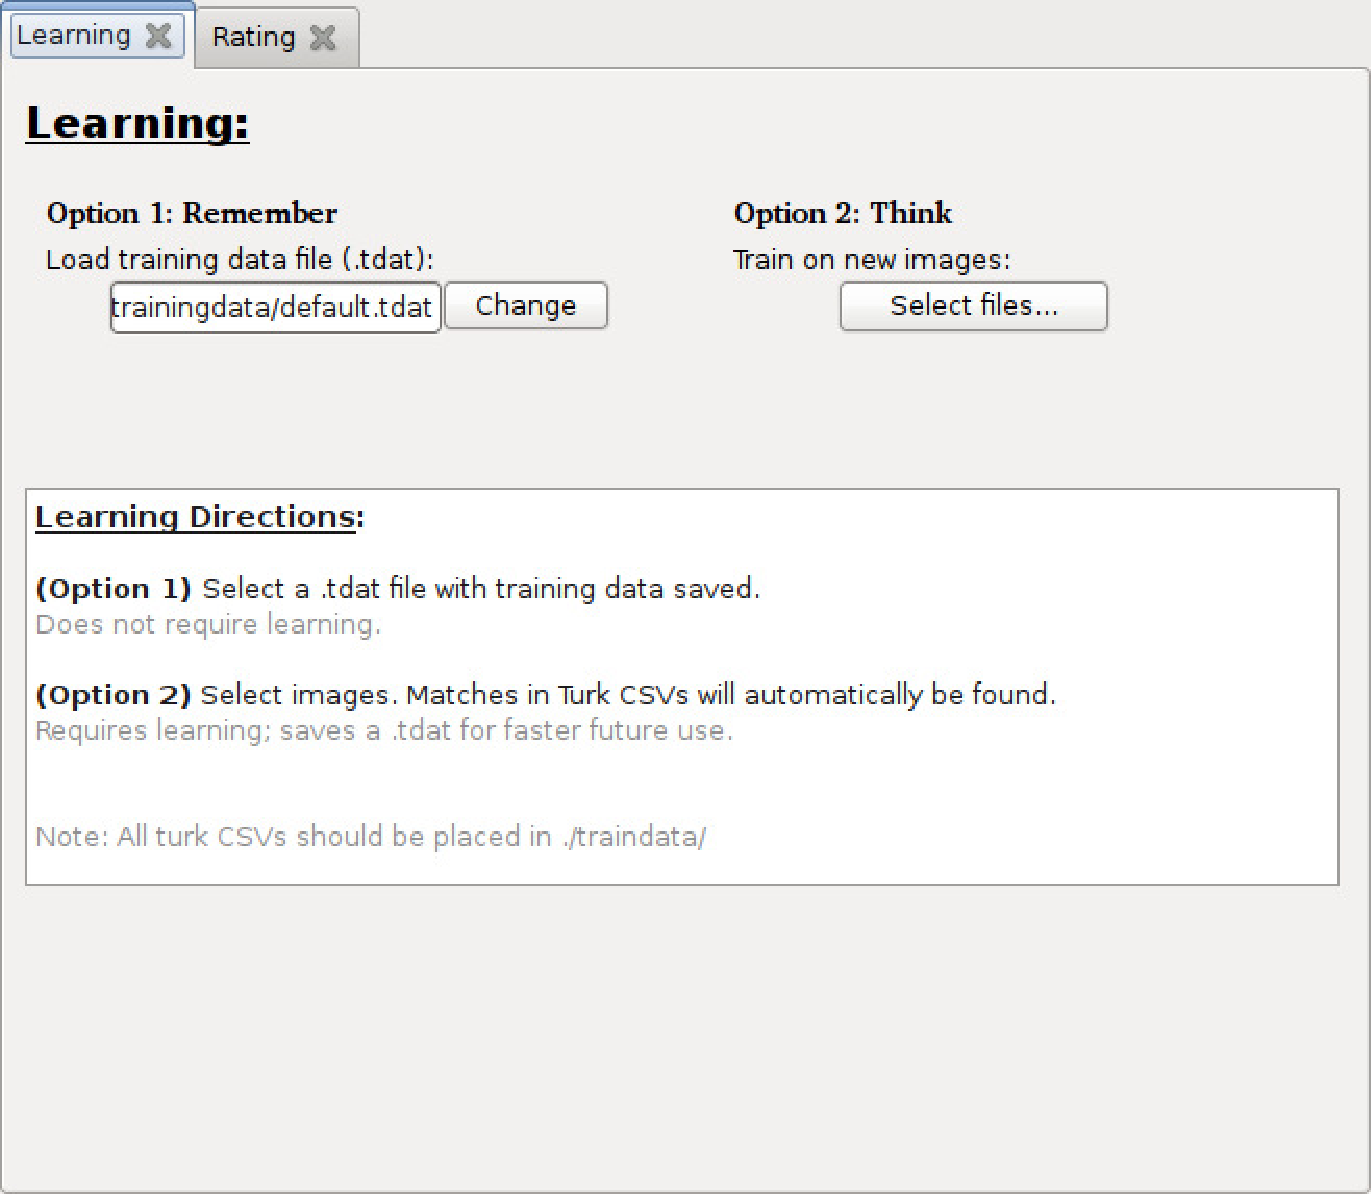
\epsfig{file=learnpage.pdf,width=15cm}
    }
  \caption{When learning, the user has two options. The first option is to choose a new set of images to train on. The second is to select saved training data.}
  \label{fig:learnpage}
\end{figure*}

\subsection{Prediction}
The user selects which images to predict on. Two outputs are produced: one with all images and their ranking (Figure \ref{fig:imagebrowser}) and one with the highest-rated images (Figure \ref{fig:topimages}).

\begin{figure*}[h!]
  \centering
    \fbox{
      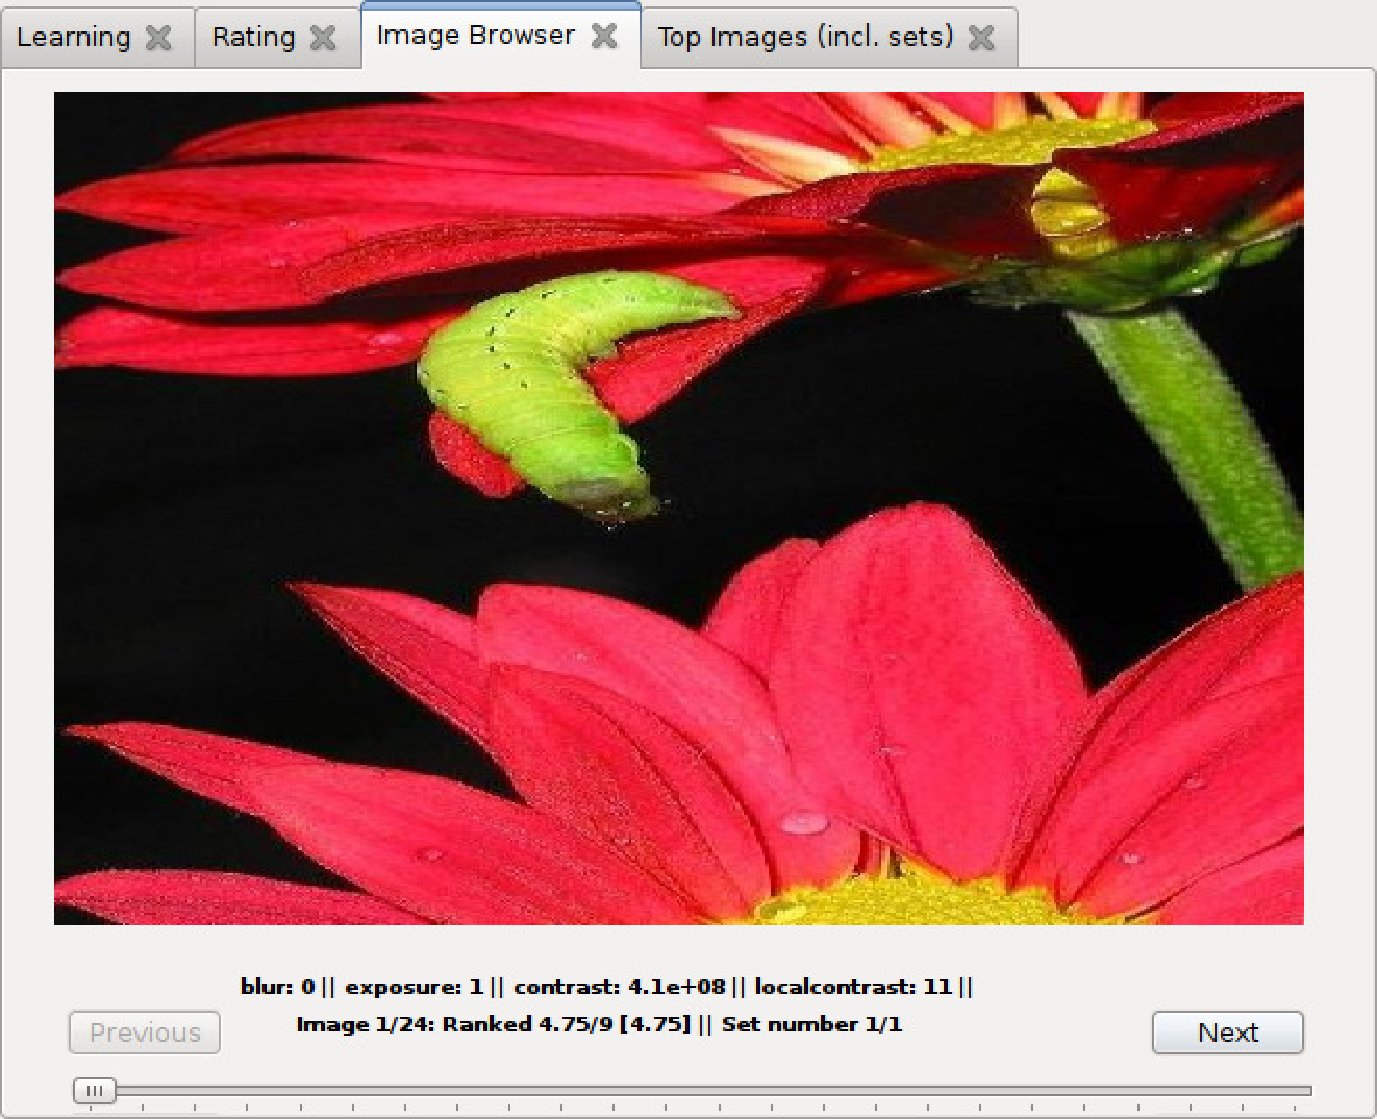
\epsfig{file=imagebrowser.pdf,width=15cm}
    }
  \caption{This interface shows the list of images with some of their low-level rankings and final prediction.}
  \label{fig:imagebrowser}
\end{figure*}

\begin{figure*}[h!]
  \centering
    \fbox{
      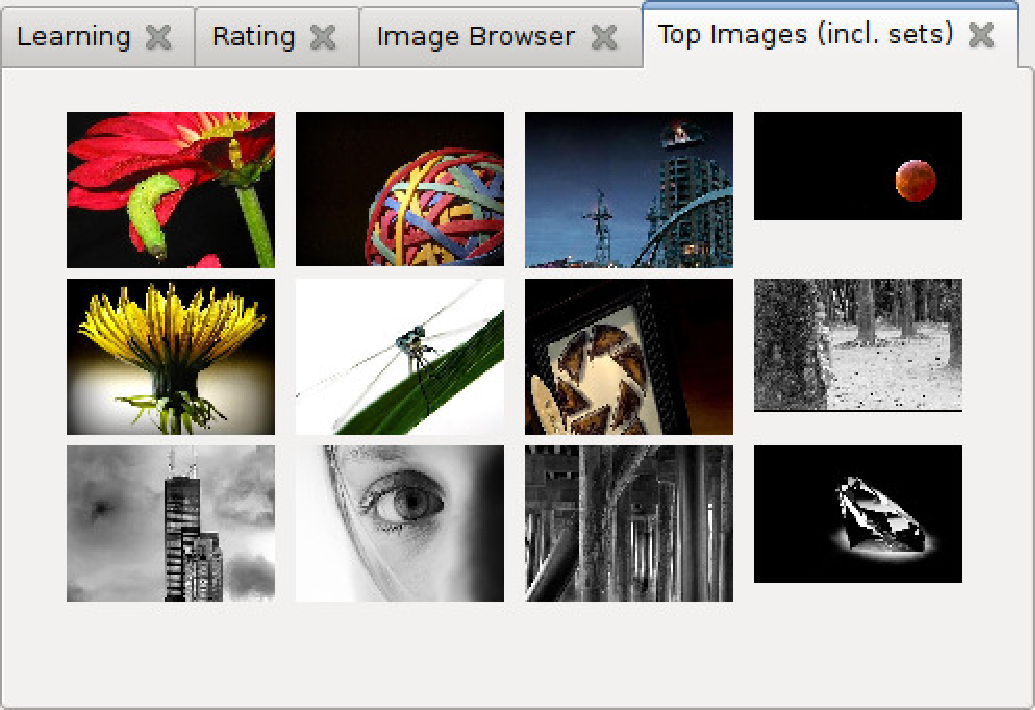
\epsfig{file=topimages.pdf,width=15cm}
    }
  \caption{This is a quick view of the top twelve images, as rated by the application.}
  \label{fig:topimages}
\end{figure*}

\section{CMPS 242: What We Completed}
This paper incorporates Machine Learning into our previous work. For full disclosure, we will list what is included in this paper that was created previously:

\begin{enumerate}
\item The low-level feature calculations and related framework (but they had been optimized for speed, allowing large training datasets).
\item The GUIs in Figures \ref{fig:imagebrowser} and \ref{fig:topimages} (but they were combined into a single interface for this paper).
\end{enumerate}

The rest of the contributions were developed solely for our final project in CMPS 242, including:
\begin{enumerate}
\item Designing Amazon Mechanical Turk tests; the framework for reading the unmodified CSVs containing Turk results; combining multiple CSVs that may ask Turkers different questions.
\item Integrating all Machine Learning techniques.
\item Making the GUI support both learning and prediction in a similar interface.
\end{enumerate}

Although we were only able to train on around 200 images, our framework allows us to quickly add more, given additional Turk data. Each picture cost \$0.05 for accurate data.

\bibliographystyle{plain}
\bibliography{README_BIB}

\end{document}
